\documentclass[conference]{IEEEtran}
\IEEEoverridecommandlockouts
% The preceding line is only needed to identify funding in the first footnote. If that is unneeded, please comment it out.
\usepackage{cite}
\usepackage{amsmath,amssymb,amsfonts}
\usepackage{algorithmic}
\usepackage{graphicx}
\usepackage{textcomp}
\usepackage{xcolor}
\usepackage{hyperref} % For hyperlinks in the PDF
\hypersetup{
    colorlinks = true
}
\usepackage{fancyvrb}
\def\BibTeX{{\rm B\kern-.05em{\sc i\kern-.025em b}\kern-.08em
    T\kern-.1667em\lower.7ex\hbox{E}\kern-.125emX}}
\begin{document}

\title{Machine Learning for Pinnacle Matchmaking in \textit{Destiny 2}\\
    % This footnote is usually used for funding; we acknowledge course staff 
    % here instead. They granted us w/ knowledge, I suppose?
    \thanks{This project was done for CS229: Machine Learning.
        The code is available on GitHub at
        \href{https://github.com/garrickf/d2-ml}{garrickf/d2-ml}.
        Thanks to Prof. Moses Charikar, Prof. Chris Ré, and the rest of the teaching team for their
        feedback on the project and a great class!}
}

\author{\IEEEauthorblockN{Garrick Fernandez}
    \IEEEauthorblockA{\textit{Department of Computer Science} \\
        \textit{Stanford University}\\
        Stanford, CA\\
        garrick@cs.stanford.edu}
}

\maketitle

\begin{abstract}
    Video games often contain online components that allow players across the world
    to interact and play with one another. The systems which perform the matching
    of players into teams are often collectively referred to as ``matchmaking.'' We
    focus on analyzing matchmaking in the video game \textit{Destiny 2}, an
    online first-person shooter developed by Bungie. In this paper, we develop and
    apply machine learning techniques to Destiny 2 game data exposed by the
    Bungie.net Platform API, with the goal of predicting the ``success'' of the
    matching of a group of player, as measured by end of game standing and time to
    activity completion. The main contributions of this paper are (1) a structured
    data pipeline for retrieving, processing and aggregating data scraped from the
    Platform API, (2) data analysis and application of machine learning for
    supervised and unsupervised tasks, and (3) explorations of and proposals for
    future work in feature engineering.
\end{abstract}

\begin{IEEEkeywords}
    Category: Finance and Commerce, video games, matchmaking, regression, data
    collection, API
\end{IEEEkeywords}

\section{Introduction and Problem Motivation}

In the realm of online gaming, \textit{Destiny 2} is unique in that it
facilitates player interaction in many ways. Players can organically encounter
each other online while exploring the game's many worlds, as well as prompt to
get matched with other players in order to participate in cooperative and
competitive activities. This latter process, a more explicit form of
matchmaking, depends on the fact that there are other players currently online
who are looking to play the same activity. However, there are some activities
that have matchmaking disabled, due to the difficulty, coordination, and
prerequisites required for the activity (these activities are referred to as
``pinnacle'' or ``aspirational'' activities—the things you do to demonstrate
mastery over the game).

This design choice has created an ecosystem around finding people to play with,
and there are already several established networks that exist for finding
teammates, such as LFG (``looking for group") websites, and clans, organized
groups of players that regularly play together. Bungie themselves have an
in-game matchmaking solution, called Guided Games, which attempts to pair solo
players (Seekers) and organized teams (Guides). Unfortunately, Guided Games has
been in beta since the game's original release in 2017 \cite{guided-games},
and it suffers from low concurrent player populations and, by extension, long
queue times \cite{problems}. The advantage of clan membership (and, to
some extent, using LFG apps) are that players can schedule activities in
advance, but these routes can be intimidating to new or introverted players.
One potential approach that could improve the experience of looking for a team
would be to use a system to recommend other players they could play an activity
with right now, or in the near future: a ``team-activity-time" recommendation.
Instead of putting the onus on a player to find a group, the system can take
advantage of the fact that many people are in similar situations, wanting to
play the same activity—and proactively match them.

As a step towards that goal, we employ a number of machine learning techniques
on data publicly accessible via the Bungie.net Platform API
\cite{api}, with the goal of evaluating the success or fitness of a
matched group of players. This system could be employed in a matchmaking
pipeline to make recommendations on which players could play an activity
together.

More formally, we define our task as a supervised learning task, where the
examples are historical games whose information we can query from the API, and
the labels are measures of ``success'' reported by the game—for example, the
time it takes to complete an activity, or the team's standing, victory or
defeat, at the end of a game.

The paper is structured as follows: In section \ref{DC}, we
outline a process for scraping data from the \textit{Destiny 2} API. In
section \ref{M}, we outline the methods we tried for learning on
our task. In section \ref{RI}, we detail the experiments we tried
and evaluate the results of our exploration. In section \ref{RW},
we situate our work and results in the existing literature. In section
\ref{CFW}, we summarize our results and discuss avenues for future
work.

\section{Data Collection}\label{DC}

Collecting data was a significant component of the project due to the nature of
its source. Traditional datasets with well-formed features are not publicly
available for \textit{Destiny 2}; however, some data is exposed via the
Bungie.net Platform API, opening the door for scraping together a dataset. The
API contains upwards of 100 endpoints that allow both first-party and
third-party apps to access and manipulate various in-game and player data.

% Yuck, had to insert a lot of filler words on this line to make it look nice
Of these many endpoints, only a subset provide any useful information for our
learning task. For example, the \texttt{Destiny2.GetPostGameCarnageReport} endpoint returns a
summary of information related with a given \texttt{activityId}, internally
referred to as a post-game carnage report (PGCR). The \texttt{activityId}
is an unsigned 64-bit integer, and it is assigned to activities in ascending
order. See Fig.~\ref{response} for an example PGCR response.

\begin{figure}[htbp]
    \begin{Verbatim}[fontsize=\small]
{
    "Response": {
        "period": "2021-05-07T10:06:12Z",
        "startingPhaseIndex": 0,
        "activityDetails": {
            "referenceId": 1575864965,
            "directorActivityHash": ...,
            "instanceId": "8400554258",
            "mode": 63,
            "modes": [
                64,
                63
            ],
            "isPrivate": false,
            "membershipType": 3
        },
        ...
    }
}
    \end{Verbatim}
    \caption{Truncated JSON PGCR response (full length is 2844 lines) for
        \texttt{activityId = 8400554258}. This is a game of Gambit (a competitive player vs.
        player mode, with additional non-player combatants (the ``environment''), often categorized as PvPvE.
        There are additional fields for player statistics and
        game metadata.}
    \label{response}
\end{figure}

Assuming we rate-limit our requests to 25 per-second (the limit imposed by the
API), querying activity information for every \texttt{activityId} from
September 2017 to the present (about 8.4 billion activities) would take upwards
of 10 years! To make things feasible, we limit our range to a period of
10K/100K activities performed starting at an arbitrary \texttt{activityId} (we picked one
for a game played around May).
We implemented a threadpool to parallelize outgoing requests, rate-limiting to
avoid throttling; this sped up data collection by up to fourteen fold.

An additional layer of complication in the data collection is the presence of
hashes in the response rather than localized English strings (see See
Fig.~\ref{response}, \texttt{directorActivityHash}). The API is
internationalized, and so the API responses are decoupled from any language,
and an additional hydration step is needed to transform hashes into localized
English strings. In particular, a manifest (a file containing metadata for a
group of accompanying files—in our case, all the data we can query from the
platform API) can be downloaded as a compressed SQLite database. The tables
therein map hashes to localized strings, representing static definitions of
objects found within \textit{Destiny}.

We wrote an additional script script to download the manifest and process it
into an index used in the data collection routine.

There is a level of stochasticity in the web scraper, as some requests time
out, network issues arise, etc. In addition, our scraper does not reattempt a
query for a failed \texttt{activityId}; as such, on one particular run of
scraping 10K activities, we got back 8789 instances and 6042 scraped attributes
(many empty), spanning 124 unique activities (see Table
\ref{tab1}). The distribution of activities are shown in
Fig.~\ref{power-dist}, Fig.~\ref{top-bot}, and
Fig.~\ref{pinned}.
%
\begin{figure}[htbp]
    \centerline{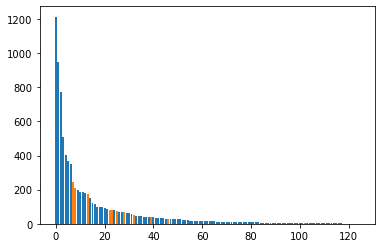
\includegraphics[width=0.75\columnwidth]{figs/activities-pwr-dist.png}}
    \caption{Distribution of activity type from 10K queries (field name:
        \texttt{directorActivityHash}); the
        activities players choose to play follows a power distribution. Activities from
        Fig.~\ref{pinned} are highlighted in orange for comparison.}
    \label{power-dist}
\end{figure}
%
\begin{figure}[htbp]
    \centerline{
        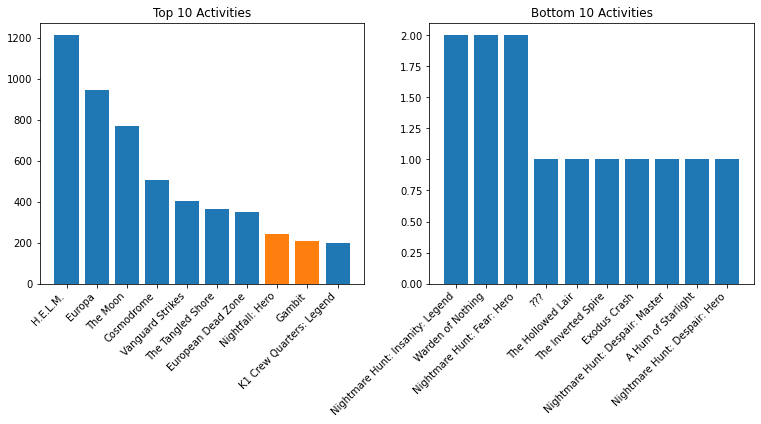
\includegraphics[width=0.95\columnwidth]{figs/top-10-and-bottom-10.png}
    }
    \caption{Distributions of the top 10 and bottom 10 activities. Popular activities are
        social spaces (``H.E.L.M.''), free roam (``Europa,'' ``The Moon,'' etc.),
        possibly because they act as hubs or places to visit before
        other, more challenging activities. Activities from
        Fig.~\ref{pinned} are highlighted in orange for comparison.}
    \label{top-bot}
\end{figure}
%
\begin{table}[htbp]
    \caption{Data Collection Results}
    \begin{center}
        \begin{tabular}{|c|c|c|c|}
            \hline
            \textbf{Scrape} & \textbf{Examples Found} & \textbf{Attributes Found} & \textbf{File Size} \\
            \hline
            10K             & 8789                    & 6042                      & 55MB               \\
            10K (Gambit)    & 223                     & 114                       & 150KB              \\
            100K            & 80026                   & 11498                     & 0.93GB             \\
            \hline
        \end{tabular}
        \label{tab1}
    \end{center}
\end{table}

We configured the scraper to filter data by game mode, as each game mode
supports a different number of players and exposes different metadata and stats
(in Gambit, for example, players seek to defeat an enemy boss, the Primeval,
that isn't present in other game modes, and thus carries unique statistics).
This has the added benefit of reducing the number of ``empty'' columns.

We focus our attention on the game mode Gambit. Due to its requirement for team
cooperation, Gambit matches are a good source of statistics for how teams
behave and work together. From our initial 10K scrape, we filtered out 223
Gambit matches, with 113 attributes per example. The relatively high number of
attributes is due to collecting statistics for each player, and there are eight
players minimum per Gambit match (sometimes, a player may leave the match, in
which case an additional player joins to fill the team).

\begin{figure}[htbp]
    \centerline{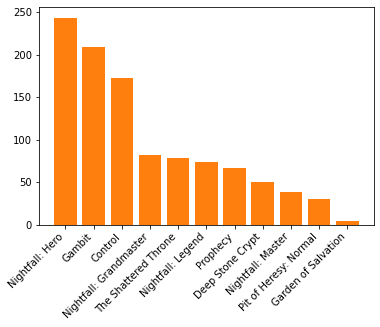
\includegraphics[width=0.75\columnwidth]{figs/pinned.png}}
    \caption{Distribution of activities selected by the author. Aside from the top
        three, all activities here do not have matchmaking by default, so recommendations would be most impactful for these pinnacle activities. Game
        modes like Gambit or Control can also serve as a good proxy, because of their competitive nature.}
    \label{pinned}
\end{figure}

\section{Methods}\label{M}
There are multiple factors of ``success'' in a single \textit{Destiny 2}
game or match. If the game mode does not contain opposing teams (player vs.
environment, or PvE), the activity completion time can be taken as a metric of
team cohesion and success. The longer the time to completion, the worse the
team did. In competitive game modes (PvP or PvPvE), there are separate
competing teams, and the standing, or end-of-game result (victory or defeat)
can be taken as a metric of team success.

In order to learn and predict completion time, we consider several methods. One
method is linear regression, whose cost function is given by:

\begin{equation}
    J(\theta) = \frac{1}{2} \sum_{i = 1}^n
    (h_\theta (x^{(i)}) - y^{(i)})^2
\end{equation}

where $h_\theta(x) = \sum_{i=0}^d \theta_i x_i =
    \theta^\top
    x$ (we use the convention of letting
$x_0 = 1$, the intercept). This function is convex. We can derive
this cost function from a probabilistic/MLE perspective. The vectorized update
rule for batch gradient descent is

\begin{equation}
    \theta := \theta + \alpha \sum_{i=1}^n
    (y^{(i)} -
    h_\theta (x^{(i)}))x^{(i)}\label{lms-update}
\end{equation}

Notice we don't normalize over the number of examples (as is convention with
neural networks). Also note that the negative sign typical in gradient descent
(we move against the direction of the gradient to minimize the cost function)
has been pushed inside the sum in \eqref{lms-update}.

As there are a lot of features, and some of them may be collinear (for example,
the number of kills versus the number of combatants defeated, i.e., kills and
assists), regularization may result in better, simpler models and less
overfitting to the training data. We consider ridge regression and lasso
regression, whose cost functions are least squares with L2 and L1
regularization, respectively. The cost function for Ridge regression is:

\begin{equation}
    J(\theta) = \frac{1}{2} \sum_{i = 1}^n
    (h_\theta (x^{(i)}) - y^{(i)})^2 + \lambda
    \|\theta\|_2
\end{equation}

Where $\lambda$ is the regularization strength. The cost function
for Lasso regression is:

\begin{equation}
    J(\theta) = \frac{1}{2} \sum_{i = 1}^n
    (h_\theta (x^{(i)}) - y^{(i)})^2 + \gamma
    \|\theta\|_1
\end{equation}

Where $\gamma$ is the regularization strength. By taking a
Bayesian interpretation of regularization, we can view ridge and lasso
regression as having a Gaussian and Laplace prior over the parameters
$\theta$, respectively. Both priors encourage the parameter
values to be closer to their mean (i.e., zero), resulting in a shrinkage
effect. In particular, lasso regression is known to result in sparse
parameters, where most parameter values are zero, and only some are non-zero.
This could be useful for identifying which features are the most useful for our
learning task.

To evaluate the methods above, we use the coefficient of determination
$R^2$, which is defined as:

\begin{equation}
    1 - \frac{u}{v}
\end{equation}

Where $u$ is the sum of squared residuals over our
validation (or test) set:

\begin{equation}
    u = \sum_{i = 1}^{n_\text{val}}
    (y^{(i)} - \hat{y}^{(i)})^2
\end{equation}

and $v$ is the total sum of squares, defined as:

\begin{equation}
    v = \sum_{i = 1}^{n_\text{val}}
    (y^{(i)} -
    \bar{y})^2\label{total-ss}
\end{equation}

where in \ref{total-ss}, $\hat{y}$ is the mean of the
observed data. Intuitively, this statistic gives some measure of the goodness
of fit for our model. The best possible $R^2$ score is 1.0.

\section{Experiments, Results and Interpretation}\label{RI}

\subsection{Tools}
In developing our data collection pipeline described in section
\ref{DC}, we used Postman \cite{postman} in order to
inspect and explore the results of API calls. The requests library was used in
order to make the calls.

We used an external library, scikit-learn \cite{sklearn}, to perform
the methods described in Section \ref{M}. Numpy and pandas were
used for data manipulation, and matplotlib was used for making visualizations.

\subsection{Regression on Activity Completion Time}

See Table \ref{tab2} for a collection of the results. We reduced
the number of features down to 81 by removing duplicate features (e.g., each
player had an activity completion time, but they were all the same). We try
both normalizing features and leaving them unnormalized. As there are different
scales of features (for example, the kills a player performs in a match, versus
points they earn, which may be on a different scale), we would expect
normalization of features to help here.

For ridge and lasso regression, we additionally performed hyperparameter search
over the regularization strength.

It appeared lasso regression with normalized features and moderate
regularization strength ($\gamma = 1$) outperformed other models on
the validation set. Notably, if the regularization strength was tuned too high,
this resulted in a poor fit to the data, even reaching 0.0 with
$\gamma = 10$ (this indicates a constant model that disregards the
input features).

Inspecting the parameters returned by the model, we find that only 13 of the 81
features are selected, and they are primarily the number of player deaths for
each of the characters. Ranked by importance, we see that number of deaths is a
primary factor in determining the length of a Gambit match (see
Fig.~\ref{lasso}).

\begin{table}[htbp]
    \caption{Regression on Activity Completion Time}
    \begin{center}
        \begin{tabular}{|c|c|c|c|c|}
            \hline
            \textbf{Method} & \textbf{Reg. Strength} & \textbf{Train $R^2$} & \textbf{Val $R^2$} & \textbf{Test $R^2$} \\
            \hline
            LinReg          & N/A$^{\mathrm{a}}$     & \textbf{0.8299}      & 0.6944             &                     \\
            LinReg$^*$      & N/A                    & 0.8268               & 0.6803             &                     \\
            \hline
            Ridge           & 0.03                   & 0.8297               & 0.6934             &                     \\
                            & 0.1                    & 0.8293               & 0.6925             &                     \\
                            & 0.3                    & 0.8285               & 0.6930             &                     \\
                            & 1                      & 0.8276               & 0.6962             &                     \\
                            & 3                      & 0.8266               & 0.6991             &                     \\
                            & 10                     & 0.8252               & 0.6978             &                     \\
            \hline
            Ridge*          & 0.03                   & 0.8252               & 0.6959             &                     \\
                            & 0.1                    & 0.8208               & 0.7115             &                     \\
                            & 0.3                    & 0.8091               & 0.7265             &                     \\
                            & 1                      & 0.7749               & 0.7371             &                     \\
                            & 3                      & 0.6984               & 0.7136             &                     \\
                            & 10                     & 0.5081               & 0.5568             &                     \\

            \hline
            Lasso           & 0.03                   & 0.8290               & 0.6935             &                     \\
                            & 0.1                    & 0.8264               & 0.6966             &                     \\
                            & 0.3                    & 0.8255               & 0.6937             &                     \\
                            & 1                      & 0.8211               & 0.6859             &                     \\
                            & 3                      & 0.8116               & 0.6418             &                     \\
                            & 10                     & 0.7885               & 0.5899             &                     \\
            \hline
            Lasso*          & 0.03                   & 0.8224               & 0.6817             &                     \\
                            & 0.1                    & 0.8153               & 0.6745             &                     \\
                            & 0.3                    & 0.7959               & 0.7135             &                     \\
                            & 1                      & 0.7253               & \textbf{0.7667}    & 0.6463              \\
                            & 3                      & 0.4121               & 0.4442             &                     \\
                            & 10                     & 0.0000               & -0.0348            &                     \\
            \hline
            \multicolumn{4}{l}{$^{\mathrm{a}}$Regularization applies only to Ridge and Lasso.}                         \\
            \multicolumn{4}{l}{$^*$Indicates normalization of features was applied.}                                   \\
        \end{tabular}
        \label{tab2}
    \end{center}
\end{table}

\begin{figure}[htbp]
    \centerline{
        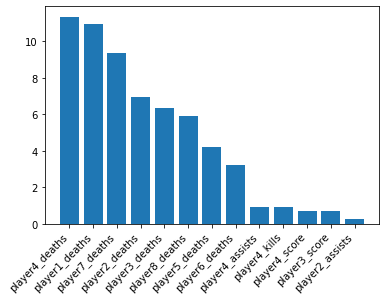
\includegraphics[width=0.75\columnwidth]{figs/lasso-model-weights.png}
    }
    \caption{Non-zero weights and attributes selected by the best lasso
        model, as evaluated using Table \ref{tab2}. Deaths are weighted more than
        other features.}
    \label{lasso}
\end{figure}

Why could this be? It turns out, there is a mechanic in Gambit called ``Death
Heals Primeval,'' where player deaths can cause the final boss to regenerate
health. This would likely have a direct impact on the length of the match, as
players would have to spend more time defeating the boss with each additional
death they incur.

\section{Related Work}\label{RW}

This project seeks to look at ways of performing machine learning on scraped
video game data in order to facilitate better matchmaking, whether between
currently online players, or as a ``recommendation'' system for all players,
online and offline, in a game's pool. The TrueMatch system, developed by Minka
and Zaykov at Microsoft Research \cite{truematch}, has the similar goal
of using AI for matchmaking. Their system uses a reinforcement learning model
in order to build a probabilistic model of the matchmaking process that can
predict increases in online player populations and adjust tolerances for
network latency and skill gap in order to reduce waiting times for players.
Skill iteslf may be measured by another system; Herbrich, Minka, and Graepel
outline an ELO-like system called TrueSkill \cite{trueskill}, a Bayesian
skill rating algorithm based on approximate message passing in factor graphs.

In contrast, our project is from the perspective of not having access to
internal data, or aggregated data over a player's history (such as skill or ELO
rankings). As such, the learning task is somewhat harder, and there are less
``good'' quality features to work with. In light of \textit{Destiny}'s
unique pinnacle activities requiring player coordination and having matchmaking
disabled, we care much more about team skill and fitness. We also note that in
the use case of offline recommendations, factors like ping (internet
connection) may not be as important as they would be in an online matchmaking
process, which TrueMatch seeks to optimize.

Other analyses of \textit{Destiny} data have been done; Bouchet has
analyzed the frequency of player activities as a function of light level (a
type of level that grows with in-game experience) \cite{data-anal}, and
some websites have more thoroughly scraped PGCRs to produce their own ELO
rankings of players, much like TrueSkill \cite{tracker}.

\section{Conclusion and Future Work}\label{CFW}

In conclusion, we outline a method for data collection on the
\textit{Destiny 2} API, giving us access to statistics on games and
players that we can attempt to learn information from. This data was then
applied to the task of determining player and team success in activities—in
particular, we took a closer look at activity completion times in the
competitive game mode Gambit as a proxy for team success. The main challenges 
were in scraping the data from the API, interpreting them as features, and 
reducing the dimensionality of the data by dropping or aggregating features.

While we found that deaths are bad for a team in Gambit, this may not be the
case in other activities. There are hundreds of activities in
\textit{Destiny 2}, each of which demand different skillsets and forms of
communication. More analysis needs to be done for other game modes in order to
make a better judgement.

For future work, we would be interested in performing feature engineering to
produce more aggregate features. This could involve combinations of existing
features, or additional scraping of the API to get more data. For example, an
approximation of player ELO scores could be obtained by querying for a player's
activity history (\texttt{Destiny2.GetActivityHistory}), and computing the number of wins,
number of kills, types of activities played, etc. In addition, the system which
scrapes data from the API could be made more robust (retrying failed requests,
caching data, etc.).

% \begin{table}[htbp]
%     \caption{Table Type Styles}
%     \begin{center}
%         \begin{tabular}{|c|c|c|c|}
%             \hline
%             \textbf{Table} & \multicolumn{3}{|c|}{\textbf{Table Column Head}}                                                         \\
%             \cline{2-4}
%             \textbf{Head}  & \textbf{\textit{Table column subhead}}           & \textbf{\textit{Subhead}} & \textbf{\textit{Subhead}} \\
%             \hline
%             copy           & More table copy$^{\mathrm{a}}$                   &                           &                           \\
%             \hline
%             \multicolumn{4}{l}{$^{\mathrm{a}}$Sample of a Table footnote.}
%         \end{tabular}
%         \label{tab1}
%     \end{center}
% \end{table}

\begin{thebibliography}{00}
    % Intro
    \bibitem{guided-games} ``Guided games: bungie help,''
    \url{https://help.bungie.net/hc/en-us/articles/360049198951-Guided-Games} (Accessed June 2021).

    \bibitem{problems} D. Friedman, ``Destiny 2’s solution for getting new
    players into raids has some major problems,'' \textit{Polygon},
    \url{https://www.polygon.com/2017/10/11/16453942/destiny-2-raid-guided-games} (Accessed June 2021).

    \bibitem{api} ``Bungie.net api,'' \url{https://bungie-net.github.io/multi/index.html} (Accessed June 2021).

    % Experiments
    \bibitem{postman} ``Postman: the collaboration platform for api
    development,'' \url{https://www.postman.com/} (Accessed June 2021).

    \bibitem{sklearn}
    ``Scikit-learn: machine learning in python,'' \url{https://scikit-learn.org/stable/} (accessed May 2021).

    \bibitem{truematch}
    ``TrueMatch matchmaking system,'' \textit{Microsoft Research},
    \url{https://www.microsoft.com/en-us/research/project/truematch/} (Accessed June 2021).

    \bibitem{trueskill} R. Herbrich, T. Minka, and T. Graepel, ``Trueskill(tm):
    a bayesian skill rating system,'' in \textit{Advances in Neural Information Processing Systems 19}, 2007, pp. 569–576.

    \bibitem{data-anal} J. Bouchet, ``Destiny user data analysis,''
    \url{https://rpubs.com/jonathanbouchet/destiny_user_data}, (accessed June 2021).

    \bibitem{tracker} ``Destiny 2 stats, leaderboards, and more! - destiny
    tracker,'' \url{https://destinytracker.com/} (Accessed June 2021).
\end{thebibliography}

\end{document}
